\documentclass[cic,tc,english]{iiufrgs}

\usepackage[utf8]{inputenc}   % pacote para acentuação
\usepackage{graphicx}         % pacote para importar figuras
\usepackage{times}            % pacote para usar fonte Adobe Times
% \usepackage{palatino}
% \usepackage{mathptmx}       % p/ usar fonte Adobe Times nas fórmulas
\usepackage[alf,abnt-emphasize=bf]{abntex2cite}	% pacote para usar citações abnt


\title{A Converter for Physically-Based Renderer Scenes}
\author{Hagemann}{Luiza de Azambuja}
\advisor[Prof.~Dr.]{Neto}{Manuel Menezes de Oliveira}

\keyword{formatação eletrônica de documentos}
\keyword{\LaTeX}
\keyword{ABNT}
\keyword{UFRGS}

\begin{document}

\maketitle

% dedicatoria
% \clearpage
% \begin{flushright}
%     \mbox{}\vfill
%     {\sffamily\itshape
%       ``If I have seen farther than others,\\
%       it is because I stood on the shoulders of giants.''\\}
%     --- \textsc{Sir~Isaac Newton}
% \end{flushright}

% agradecimentos
%\chapter*{Acknowledgements}


% resumo na língua do documento
\begin{abstract}
    Este documento é um exemplo de como formatar documentos para o
    Instituto de Informática da UFRGS usando as classes \LaTeX\
    disponibilizadas pelo UTUG\@. Ao mesmo tempo, pode servir de consulta
    para comandos mais genéricos. \emph{O texto do resumo não deve
      conter mais do que 500 palavras.}
\end{abstract}

% resumo na outra língua
% como parametros devem ser passados o titulo e as palavras-chave na outra 
língua, separadas por vírgulas
\begin{englishabstract}{Using \LaTeX\ to Prepare Documents at 
II/UFRGS}{Electronic document preparation. \LaTeX. ABNT. UFRGS}
    This document is an example on how to prepare documents at II/UFRGS
    using the \LaTeX\ classes provided by the UTUG\@. At the same time, it
    may serve as a guide for general-purpose commands. \emph{The text in
      the abstract should not contain more than 500~words.}
\end{englishabstract}

% lista de figuras
% \listoffigures

% lista de tabelas
% \listoftables

% lista de abreviaturas e siglas
\begin{listofabbrv}{PBR}
    \item[PBR] Physically-based Rendering
    \item[PB] Physically-based
\end{listofabbrv}

% idem para a lista de símbolos
% \begin{listofsymbols}{$\alpha\beta\pi\omega$}
%     \item[$\sum{\frac{a}{b}}$] Somatório do produtório
%     \item[$\alpha\beta\pi\omega$] Fator de inconstância do resultado
% \end{listofsymbols}

% sumario
\tableofcontents

% capitulos
\chapter{Introduction}
\section{Physically Based Rendering}
Ever since the development of modern Computer Graphics, one of the goals 
researchers aspired to was being able to synthesize images indistinguishable 
from real photographs. In order to produce physically accurate images, the 
process of image synthesis - also called \textbf{rendering} - simmulates the 
interaction of light with the representation of a three-dimensional scene. 
\textbf{Physically-Based Rendering} (PBR) is a complex process that requires 
thorough knowledge of optics, material properties, geometry and light 
propagation.

Over the years, PBR became quite popular and was widely incorporated into the 
entertainment industries. From movies to videogames, from ads to interior 
design (and bearing the need of high computational power), PBR made it possible 
for artists to bring their creations and their vision one step closer to 
reality. Today, we can say that many - if not most - algorithms used in 
computer animation, geometric modeling and texturing require that their results 
be passed through some sort of rendering process. 

As PBR popularity grew, a brand new market opened up for physically-based (PB) 
renderers. Following the creation of PBRT and the publishing of 
\textit{"Physically Based Rendering: From Theory to Implementation"},
several other research-oriented renderers were created. One of the most popular 
ones, \textit{Mitsuba}, places strong emphasis on experimental rendering 
techniques.

Following the lead of Pixar's \textit{Renderman}, many commercial and 
performance-oriented renderers appeared on the market. Focused on animation 
techniques and rendering visual effects for feature films, these renderers
provide well-established, stable rendering techniques. These renderers, such as 
\textit{LuxRender} and \textit{Octane}, are state-of-the-art renderers used by 
the animation and gaming industries.
%https://www.blenderguru.com/articles/render-engine-comparison-cycles-vs-giants

<section closing paragraph>

\section{Rendering a Scene}
% - the scene
The process of rendering an image usually starts with a scene. But what defines 
a scene? In PBR, a scene is a collection of descriptions: of the scene's 
geometry (the objects), of the objects' materials and textures, of the light 
sources and of the rendering techniques the user would like to use to form the 
image. This description is then read and interpreted by the renderer, and the 
scene is then processed into an output image.

% - stating the problem/motivation: making scenes is hard 
% (reference: http://www.laubwerk.com/home/)
But even with the vast array of softwares at our disposal, creating scenes is 
still a complex process. For instance, scenes created for architecture or 
design-oriented softwares often compile hundreds of 3D models and dozens of 
customized materials and textures, as shown in Figure 
\ref{fig:intro_complexScene}. Each material and texture has to be carefully 
defined, taking into account the target 
renderer's limitations and particularities. Crafting such scenes is an onerous, 
time-consuming effort: so much that 

\begin{figure}[h]
  
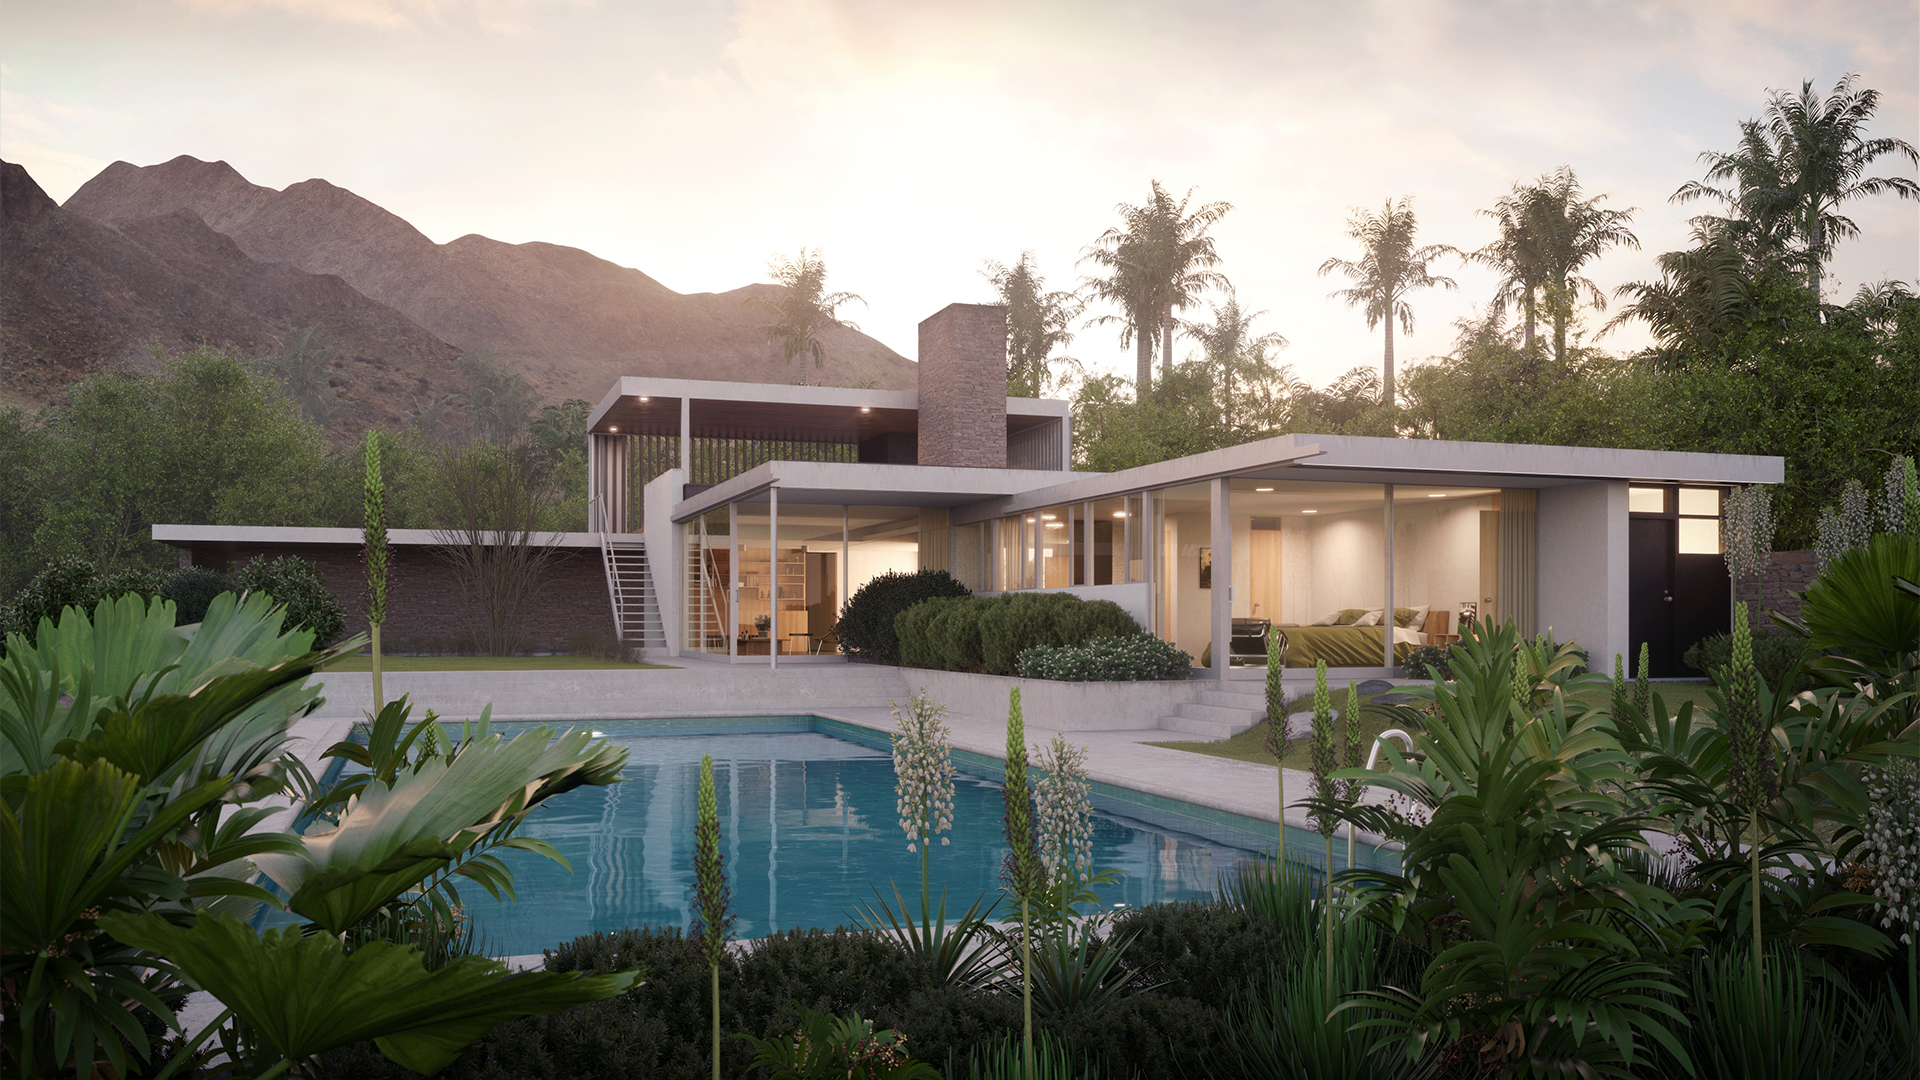
\includegraphics[width=\textwidth,height=\textheight,keepaspectratio]{../images/1_introduction/Laubwerk-Kit-12_Bauclassroom-Exterior}
  \caption{An example of a complex scene created by Laubwerk Plants Kits}
  \label{fig:intro_complexScene}
\end{figure}

% - converting a scene - what it takes
<CONVERTING A SCENE>

% - a solution proposal

\chapter{Related Works}
% - collada

% - bitterli

% - render toolbox4 
(https://github.com/RenderToolbox/RenderToolbox4/wiki/Overview)

\chapter{Theoretical Foundations}
\chapter{Project}
\chapter{Result Analysis}
\chapter{Conclusion}

% referências
% aqui será usado o environment padrao `thebibliography'; porém, sugere-se
% seriamente o uso de BibTeX e do estilo abnt.bst (veja na página do
% UTUG)

\bibliographystyle{abntex2-alf}
\bibliography{biblio}

\end{document}
